\documentclass[12pt, letterpaper]{article}

% ==========================================
%              DOCUMENT PACKAGES
% ==========================================

% --- Core Language & Encoding ---
\usepackage[english]{babel} % Sets the language and regional settings for English documents
\usepackage[utf8]{inputenc} % Allows the use of UTF-8 characters in the document
\usepackage[T1]{fontenc} % Specifies the font encoding
\usepackage[margin=1.5cm]{geometry} % Sets the page margins

% --- Colors & Graphics ---
\usepackage[table,dvipsnames]{xcolor} % Advanced color management
% \usepackage{color} % Basic package for text and background colors
\usepackage{graphicx} % Enhanced support for including external images and scaling them
\usepackage{adjustbox} % Adjusts the size, scaling, and alignment of boxes, images, and tables
% \usepackage{background} % Allows adding background images or watermarks to pages
\usepackage{float} % Improves the interface for floating objects and adds the [H] placement
\usepackage{pdflscape} % Makes landscape pages display correctly on screen in PDF viewers
\usepackage{pdfpages} % Allows the inclusion of external multi-page PDF documents

% --- Math, Science & Engineering ---
\usepackage{amsfonts} % Provides extended mathematical fonts
\usepackage{amsmath} % Provides advanced mathematical typesetting and environments
\usepackage{amssymb} % Provides extended mathematical symbols
% \usepackage{amsmath, amssymb} % (Redundant combination line omitted for stability)
\usepackage{amsthm} % Facilitates the creation of theorem-like environments
\usepackage{mathtools} % Enhances amsmath with additional math tools and bug fixes
\usepackage{thmtools} % Extensions and customization options for theorem environments
\usepackage{nicematrix} % Enhances matrices and tabulars using PGF/TikZ
\usepackage{xy} % Typesets complex graphs and diagrams
\usepackage{circuitikz} % Allows drawing of electrical networks and circuits

% --- Typography & Fonts ---
\usepackage{avant} % Sets the default sans-serif font to Avant Garde
\usepackage{cantarell} % Sets the default sans-serif font to Cantarell
\usepackage{charter} % Sets the default roman font to Charter
\usepackage{cmbright} % Sets the font family to Computer Modern Bright 
\usepackage{helvet} % Sets the default sans-serif font to Helvetica
\usepackage{inconsolata} % Sets the default typewriter (monospace) font to Inconsolata
\usepackage{iwona} % Sets the font family to Iwona 
\usepackage{kurier} % Sets the font family to Kurier 
\usepackage{lmodern} % Loads the Latin Modern fonts 
\usepackage{textcomp} % Provides additional text symbols
\usepackage{ulem} % Provides various types of text underlining and strikethroughs

% --- Tables & Lists ---
\usepackage{array} % Extends the array and tabular environments
\usepackage{arydshln} % Allows dashed lines in arrays and tables
\usepackage{bigstrut} % Adds custom vertical space in table rows
\usepackage{booktabs} % Enhances the quality of tables with better horizontal rules
% \usepackage{colortbl} % Allows coloring of rows, columns, and individual cells in tables
\usepackage{diagbox} % Creates table cells with diagonal lines 
\usepackage{enumitem} % Provides advanced control over list environments
\usepackage{longtable} % Allows tables to break across multiple pages
\usepackage{multirow} % Allows individual table cells to span across multiple rows
\usepackage{tabularx} % Creates tables with dynamically adjustable-width columns
\usepackage{pgfplotstable} % Reads and cleanly formats numerical tables directly from CSV

% --- Formatting, Layout & UI ---
\usepackage{blindtext} % Generates dummy text for testing document layouts
\usepackage{caption} % Customizes captions in floating environments
\usepackage{comment} % Allows you to block out large sections of text
\usepackage{emptypage} % Automatically removes headers and footers on empty pages
\usepackage{fancyhdr} % Allows complete customization of headers and footers
\usepackage{fancyvrb} % Enhanced verbatim environments for writing raw code
\usepackage{framed} % Creates framed, shaded, or differently highlighted text regions
\usepackage{fullpage} % Quickly sets all page margins to 1 inch
\usepackage{lipsum} % Generates Lorem Ipsum dummy text
\usepackage{mdframed} % Creates highly customizable framed environments
\usepackage{multicol} % Allows intermixing single and multiple text columns
\usepackage{parskip} % Replaces standard paragraph indentation with vertical spacing
\usepackage{setspace} % Controls line spacing (single, one-and-a-half, double)
\usepackage{subcaption} % Supports sub-figures and sub-tables with independent captions
% \usepackage{subfig} % Older package for sub-figures (subcaption is generally preferred now)
\usepackage{tcolorbox} % Creates heavily customized colored and framed text boxes
\usepackage{titlesec} % Customizes the formatting of section, subsection, and chapter headings
\usepackage{titling} % Provides advanced control over the typesetting of the document title

% --- Bibliographies & References ---
\usepackage{biblatex} % Advanced, modern bibliographic processing and formatting
\usepackage{csquotes} % Context-sensitive quotation facilities
\usepackage{makeidx} % Supports the generation of a document index
% \usepackage{natbib} % Flexible bibliography support, particularly for author-year citation styles

% --- TikZ & Plotting ---
\usepackage{tikz} % Advanced package for creating vector graphics and diagrams programmatically
\usepackage{pgf-pie} % Draws pie charts programmatically using PGF/TikZ
\usepackage{pgfplots} % Creates high-quality mathematical plots, charts, and graphs
% \usepackage{fancytikzposter} % Used to create large format academic posters using TikZ

% --- URLs & Hyperlinks ---
\usepackage{url} % Formats and properly hyphenates long URLs
\usepackage{breakurl} % Allows line breaks in URLs, especially when compiled with latex -> dvips
\usepackage{hyperref} % Creates cross-referencing, clickable links, and PDF bookmarks

% --- Code Formatting ---
\usepackage{listings} % Typesets programming source code with formatting and syntax highlighting


% ==========================================
%           DOCUMENT CONFIGURATION
% ==========================================

% Custom color definitions
\definecolor{mygray}{gray}{0.9}

% Hyperlink configuration
\hypersetup{
    colorlinks=true,
    linkcolor=blue,
    urlcolor=blue
}

% Configuración adicional para breaks en URLs
\def\UrlBreaks{\do\/\do-\do_\do.\do=\do?\do\&}
\expandafter\def\expandafter\UrlBreaks\expandafter{\UrlBreaks\do\a\do\b\do\c\do\d\do\e\do\f\do\g\do\h\do\i\do\j\do\k\do\l\do\m\do\n\do\o\do\p\do\q\do\r\do\s\do\t\do\u\do\v\do\w\do\x\do\y\do\z}

%Uncomment the following lines to use a sans-serif font
\renewcommand{\familydefault}{\sfdefault}

% TikZ libraries
\usetikzlibrary{shapes.geometric, positioning, decorations.pathreplacing}

\graphicspath{ {./img/} } % Sets the path for the graphics

\newlist{biblio}{enumerate}{1}
\setlist[biblio,1]{label=[\arabic*]}

\makeindex

% \tiny
% \scriptsize
% \footnotesize
% \small
% \normalsize (default size)
% \large
% \Large
% \LARGE
% \huge
% \Huge


% ==========================================
%         GLOBAL LISTINGS SETTINGS
% ==========================================
\lstset{
	basicstyle=\ttfamily\small,
	numbers=left,
	numberstyle=\tiny\color{gray},
	stepnumber=1,
	numbersep=10pt,
	backgroundcolor=\color{white},
	showspaces=false,
	showstringspaces=false,
	breaklines=true,
	frame=single,
	tabsize=2, 
    captionpos=b, 
    lineskip=-1pt,
	extendedchars=true,
	literate={á}{{\'a}}1 {é}{{\'e}}1 {í}{{\'i}}1 {ó}{{\'o}}1 {ú}{{\'u}}1 {Á}{{\'A}}1 {É}{{\'E}}1 {Í}{{\'I}}1 {Ó}{{\'O}}1 {Ú}{{\'U}}1 {ñ}{{\~n}}1 {Ñ}{{\~N}}1 {¿}{{\textquestiondown}}1 {¡}{{\textexclamdown}}1
}

% ==========================================
%            LANGUAGE: SQL
% ==========================================
\lstdefinestyle{sqlstyle}{
	language=SQL,
	keywordstyle=\color{blue}\bfseries,
	commentstyle=\color[rgb]{0,0.5,0}\itshape,
	stringstyle=\color{red}
}

% ==========================================
%            LANGUAGE: VHDL
% ==========================================
\lstdefinelanguage{VHDL}{
	morekeywords={entity, architecture, signal, port, in, out, inout, begin, end, process, if, then, else, elsif, case, when, others, for, while, loop, wait, library, use, std_logic, std_logic_vector, integer, boolean, rising_edge, falling_edge, component, generic, map, downto, to, and, or, not, xor, nand, nor, xnor},
	morecomment=[l]{--},
	morestring=[b]",
	sensitive=false,
	alsoletter={_}
}

\lstdefinestyle{vhdl}{
	language=VHDL,
	keywordstyle=\color{blue}\bfseries,
	commentstyle=\color[rgb]{0,0.6,0}\itshape,
	stringstyle=\color{red}
}

% ==========================================
%              LANGUAGE: C
% ==========================================
\lstdefinestyle{cstyle}{
	language=C,
	keywordstyle=\color{blue}\bfseries,
	keywordstyle=[2]\color{ForestGreen}\bfseries,
	keywordstyle=[3]\color{orange}\bfseries,
	commentstyle=\color[rgb]{0,0.5,0}\itshape,
	stringstyle=\color{red},
	directivestyle=\color{purple},
	morekeywords=[2]{uint8_t,uint16_t,uint32_t,int32_t,size_t,bool,esp_err_t,\
		httpd_handle_t,httpd_req_t,httpd_ws_frame_t,wifi_config_t,\
		wifi_init_config_t,adc_oneshot_unit_handle_t,i2c_config_t},
	morekeywords=[3]{ESP_OK,ESP_ERR_NO_MEM,HTTP_GET,HTTPD_WS_TYPE_TEXT,\
		WIFI_MODE_STA,WIFI_MODE_AP,WIFI_IF_STA,WIFI_IF_AP,ADC_CHANNEL_5,\
		WIFI_AUTH_WPA2_PSK,CONFIG_HTTPD_WS_SUPPORT},
	emph={app_main,esp_wifi_init,esp_wifi_start,esp_wifi_set_mode,\
		esp_wifi_set_config,esp_netif_init,esp_netif_create_default_wifi_sta,\
		esp_netif_create_default_wifi_ap,adc_oneshot_read,httpd_start,\
		httpd_register_uri_handler,httpd_ws_recv_frame,httpd_ws_send_frame_async,\
		u8g2_ClearBuffer,u8g2_DrawStr,u8g2_SendBuffer},
	emphstyle=\color{Magenta},
    tabsize=4 % Overrides the global tabsize of 2 for C code specifically
}

% ==========================================
%             LANGUAGE: C++
% ==========================================
\lstdefinestyle{cppstyle}{
	language=C++,
	keywordstyle=\color{blue}\bfseries,
	commentstyle=\color[rgb]{0,0.5,0}\itshape,
	stringstyle=\color{red},
	directivestyle=\color{purple},
    tabsize=4
}

% ==========================================
%           LANGUAGE: PYTHON
% ==========================================
\lstdefinestyle{pythonstyle}{
	language=Python,
	keywordstyle=\color{blue}\bfseries,
	commentstyle=\color[rgb]{0,0.5,0}\itshape,
	stringstyle=\color{red},
    % Python relies heavily on indentation, so keeping tabsize aligned is important
    tabsize=4
}

% ==========================================
%             LANGUAGE: BASH
% ==========================================
\lstdefinestyle{bashstyle}{
	language=bash,
	keywordstyle=\color{blue}\bfseries,
	commentstyle=\color[rgb]{0,0.5,0}\itshape,
	stringstyle=\color{red},
    % Bash variables often use $, so we can highlight them dynamically if needed
    moredelim=[s][\color{orange}]{\$\{}{\}}
}

% ==========================================
%           LANGUAGE: ASSEMBLY
% ==========================================
\lstdefinestyle{asmstyle}{
	language=[x86masm]Assembler,
	keywordstyle=\color{blue}\bfseries,
	commentstyle=\color[rgb]{0,0.5,0}\itshape,
	stringstyle=\color{red},
    % Adding common ARM/Microcontroller instructions for better highlighting
    morekeywords={ldr, str, mov, cmp, add, sub, b, bl, bx, push, pop, svc, eor, and, orr, lsl, lsr}
}

% % Configure header
\setlength{\headheight}{28pt} % Adjust header height for two-line header
\pagestyle{fancy}
\fancyhf{} % Clear all header and footer fields
\lhead{\textbf{Nombre:} Ugartechea González Luis Antonio -- 320223822 \\ \textbf{Asignatura:} <asignatura>, \textbf{Grupo:} <grupo>}
\renewcommand{\headrulewidth}{0.4pt}

\begin{document}

\newgeometry{margin=1.5cm}
\begin{titlepage}
    \noindent
    \renewcommand{\arraystretch}{1.5}
    % Definimos la tabla principal con dos columnas exactamente iguales (50/50)
    \begin{tabularx}{\textwidth}{|>{\centering\arraybackslash}X|>{\centering\arraybackslash}X|}
        \hline
        % Fila superior: Combinamos las dos columnas e insertamos una sub-tabla
        \multicolumn{2}{|@{}c@{}|}{%
            \begin{tabularx}{\dimexpr\textwidth-2\arrayrulewidth\relax}{m{3.5cm}|>{\centering\arraybackslash}X}
                \centering \vspace{0.2cm} 
\includegraphics[width=2cm,height=2.5cm]{escudoFI_color.png} & \large \textbf{Fundamentos de Sistemas Embebidos}
            \end{tabularx}%
        } \\
        \hline
        % Fila inferior: Alineada a la mitad exacta
        \large Facultad de Ingeniería & \large UNAM \\
        \hline
    \end{tabularx}

    \vspace{0.5cm}

    \begin{center}
        {\fontsize{35}{48}\selectfont Laboratorio de Fundamentos de} \\
        {\fontsize{35}{48}\selectfont Sistemas Embebidos\par}
        % Línea divisoria azul (se puede ajustar el tono de azul)
        \textcolor{MidnightBlue!70}{\rule{\textwidth}{1pt}}
    \end{center}

    \vspace{2cm}

    \begin{center}
        % Aumenta el espaciado entre filas para que coincida con el formato
        % \renewcommand{\arraystretch}{1.8}
        \fontsize{15}{21}\selectfont
        % Columna 1: Alineada a la derecha, en cursiva (itshape) y de 4.5cm de ancho
        % Columna 2: Alineada a la izquierda
        \begin{tabular}{>{\raggedleft\arraybackslash\itshape}p{4.5cm} @{\hspace{0.5cm}} l}
            Profesor(a): & \underline{\makebox[10cm][l]{ Eduardo Fragoso Navarro}} \\
            Asignatura: & \underline{\makebox[10cm][l]{ Fundamentos de Sistemas Embebidos}} \\
            Grupo: & \underline{\makebox[10cm][l]{3}} \\
            No de Práctica(s): & \underline{\makebox[10cm][l]{5}} \\
            Integrante(s): & \underline{\makebox[10cm][l]{Tepal Briseño Hansel Yael - 320078282}} \\
            & \underline{\makebox[10cm][l]{Ugartechea González Luis Antonio - 320223822}} \\
            No. de brigada: & \underline{\makebox[10cm][l]{12}} \\
            Semestre: & \underline{\makebox[10cm][l]{ 9\(^\circ\)}} \\
            Fecha de entrega: & \underline{\makebox[10cm][l]{6 de octubre de 2026}} \\
            Observaciones: & \underline{\makebox[10cm][l]{}} \\
            & \underline{\makebox[10cm][l]{}} \\
        \end{tabular}
    \end{center}

\end{titlepage}
\restoregeometry

\newpage
\fontsize{25}{21}\selectfont CALIFICACIÓN: \underline{\makebox[10cm][l]{}}
\newpage
\normalsize

\section*{\centering \fontsize{14}{17}\sffamily\selectfont Servidor web en el ESP32}

\section*{\centering \fontsize{14}{17}\sffamily\selectfont Objetivos}

El objetivo de esta práctica fue implementar un servidor web sobre la tarjeta
XIAO ESP32-S3 para supervisar remotamente, mediante una conexión WiFi, la
lectura de un potenciómetro y enviar mensajes a una pantalla OLED. Para ello se
integraron la lectura analógica mediante el ADC1, la comunicación inalámbrica
WiFi en modo punto de acceso (AP) y una comunicación bidireccional mediante
WebSocket. También se consideró que el sistema puede operar en modo estación
(STA), conectándose a una red WiFi existente.

También se buscó comprender la diferencia entre una petición HTTP convencional
y una conexión persistente WebSocket. La página se entrega inicialmente
mediante HTTP y, una vez cargada, recibe automáticamente las mediciones del ADC
por la ruta \texttt{/ws}; de forma inversa, el texto escrito en el navegador se
transmite por esa misma conexión para visualizarse en la OLED.

\section*{\centering \fontsize{14}{17}\sffamily\selectfont Resultados y análisis}

\subsection*{\fontsize{12}{17}\sffamily\selectfont Ejercicio 1: Circuito}

Se armó el circuito con un potenciómetro y una pantalla OLED conectada al bus
I2C de la tarjeta. El potenciómetro se conectó al pin D5, correspondiente al
GPIO 6 y al canal 5 del ADC1. La pantalla utilizó D8 (GPIO 7) como SDA y D7
(GPIO 44) como SCL. En el programa se configuró el ADC con una resolución de 12
bits, por lo que las lecturas se encuentran en el intervalo de 0 a 4095.

\begin{figure}[H]
    \centering
    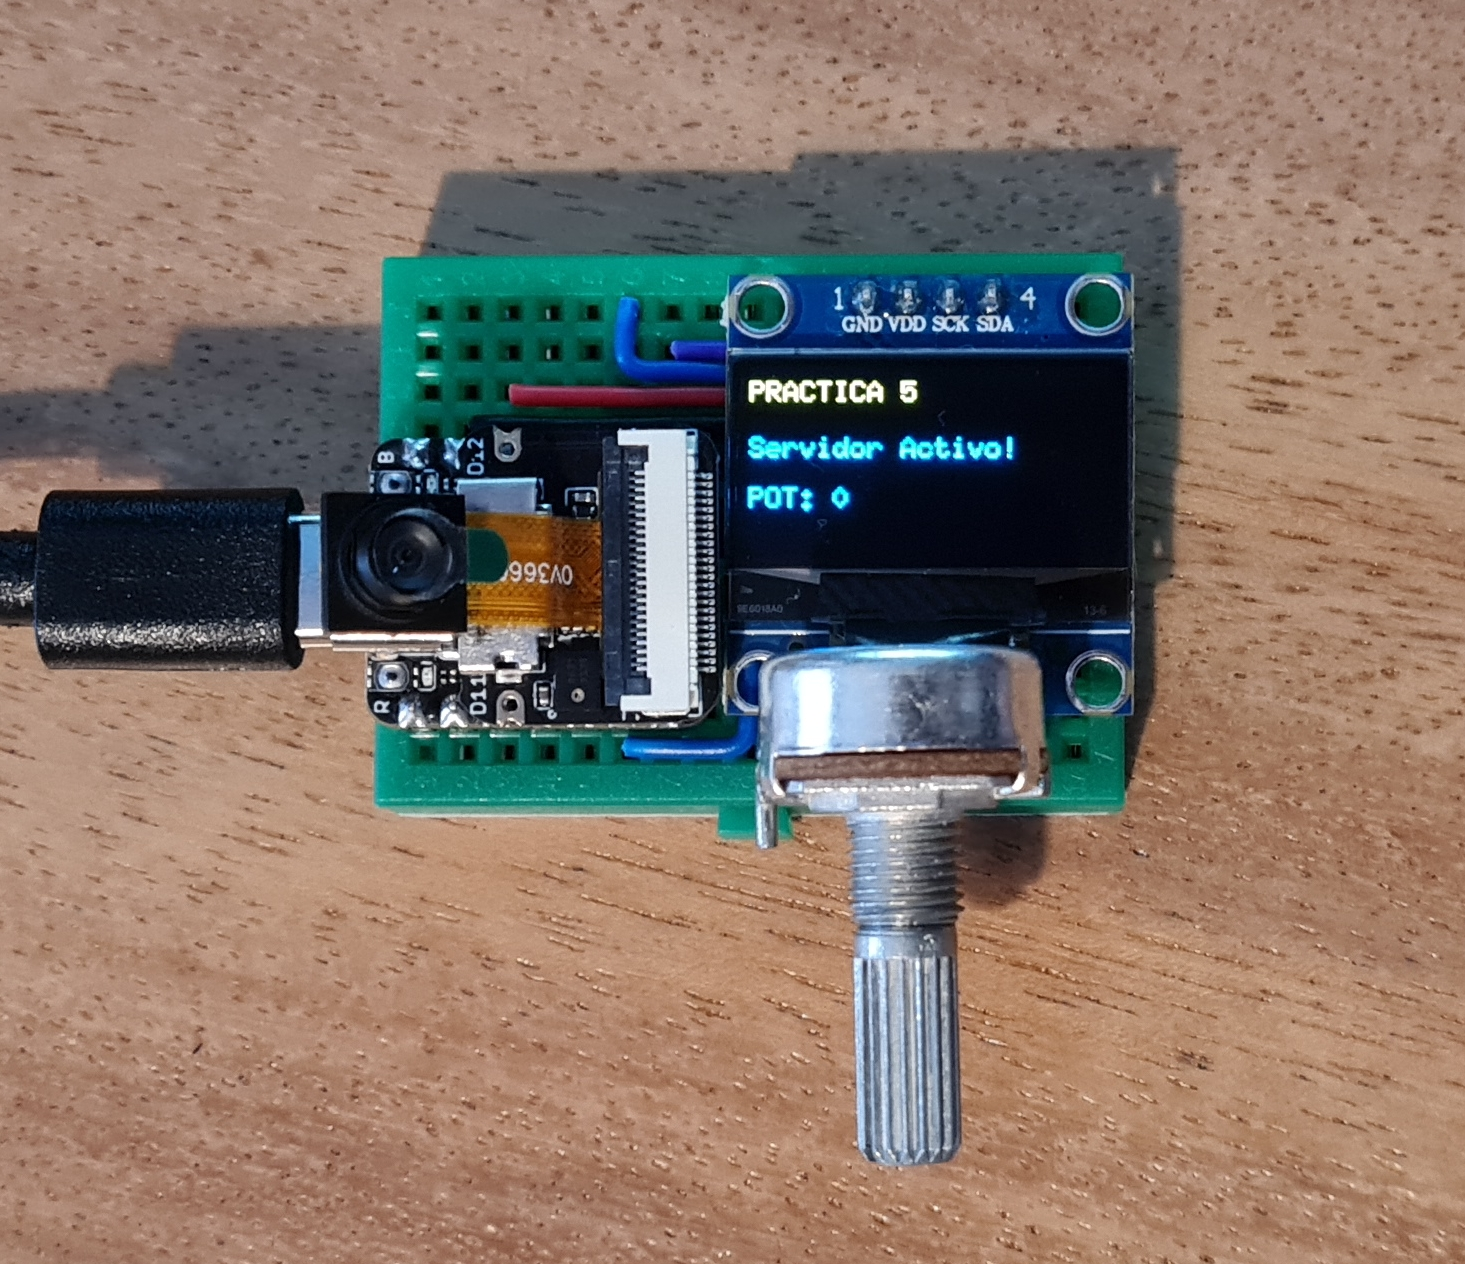
\includegraphics[width=0.35\textwidth]{esp_01.jpg}
    \caption{Circuito implementado y pantalla OLED con el servidor activo.}
    \label{fig:circuito}
\end{figure}

La pantalla OLED se controló mediante la biblioteca U8g2 y una implementación
de las funciones de transferencia I2C. Esto permitió actualizar en la misma
pantalla el estado del servidor, el mensaje recibido y el valor actual del
potenciómetro.

\subsection*{\fontsize{12}{17}\sffamily\selectfont Ejercicio 2: Funcionamiento del sistema}

La implementación inalámbrica se realizó por ambos métodos mediante WiFi y modo
de red AP (punto de acceso). Por cuestiones de facilidad de configuración y
estabilidad durante las pruebas, el ESP32 creó la red \texttt{ESP32-S3} con la
contraseña \texttt{12345678}, mientras que el navegador se conectó directamente
a la dirección \texttt{192.168.4.1}. Esta alternativa permitió realizar la
práctica sin depender de un router externo. La evidencia de la terminal
confirma la creación del punto de acceso y la dirección que debe abrirse en el
navegador.

\begin{figure}[H]
    \centering
    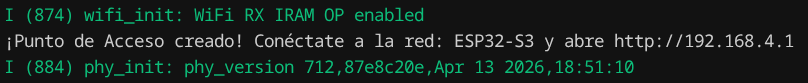
\includegraphics[width=0.82\textwidth]{ap_ip.png}
    \caption{Creación del punto de acceso y dirección IP del ESP32.}
    \label{fig:ap_ip}
\end{figure}

\begin{figure}[H]
    \centering
    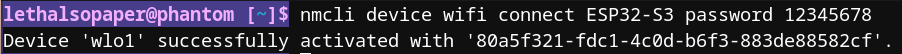
\includegraphics[width=0.82\textwidth]{connection.png}
    \caption{Conexión de la computadora a la red inalámbrica del ESP32.}
    \label{fig:connection}
\end{figure}

La modalidad de conexión se selecciona en el código mediante la constante
\texttt{WIFI\_MODE\_SELECTION}. El valor cero selecciona el modo estación
(STA), mientras que un valor diferente de cero selecciona el modo punto de
acceso (AP). De esta forma, ambas configuraciones utilizan el mismo servidor
web y solo cambia la forma en que se establece la red WiFi.

\begin{lstlisting}[style=cstyle, caption={Selección entre WiFi STA y punto de acceso AP}, label={lst:seleccion-wifi}]
#define WIFI_MODE_SELECTION 1

#if WIFI_MODE_SELECTION == 0
    // Modo estacion: conectarse a una red WiFi existente
#else
    // Modo AP: crear una red WiFi propia
#endif
\end{lstlisting}

Cuando se selecciona STA, el ESP32 crea una interfaz de estación, registra los
eventos de WiFi y configura el SSID y la contraseña del router. Después de
iniciar el periférico, el evento \texttt{WIFI\_EVENT\_STA\_START} solicita la
conexión y, al recibirse \texttt{IP\_EVENT\_STA\_GOT\_IP}, se imprime la
dirección asignada por el router. El navegador debe conectarse a esa misma red
y abrir dicha dirección.

\begin{lstlisting}[style=cstyle, caption={Configuración de la conexión WiFi en modo STA}, label={lst:wifi-sta}]
esp_netif_create_default_wifi_sta();
wifi_init_config_t cfg = WIFI_INIT_CONFIG_DEFAULT();
esp_wifi_init(&cfg);

wifi_config_t wifi_config = {
    .sta = {
        .ssid = WIFI_SSID,
        .password = WIFI_PASS,
    },
};

esp_wifi_set_mode(WIFI_MODE_STA);
esp_wifi_set_config(WIFI_IF_STA, &wifi_config);
esp_wifi_start();
\end{lstlisting}

En modo AP, el ESP32 crea su propia red inalámbrica en lugar de buscar un
router. Se configura el nombre de la red, la contraseña, el número máximo de
clientes y el método de autenticación. Al iniciar WiFi, la interfaz utiliza la
dirección predeterminada \texttt{192.168.4.1}; por ello el navegador se conecta
a la red \texttt{ESP32-S3} y solicita la página mediante esa dirección.

\begin{lstlisting}[style=cstyle, caption={Configuración del punto de acceso WiFi}, label={lst:wifi-ap}]
esp_netif_create_default_wifi_ap();
wifi_init_config_t cfg = WIFI_INIT_CONFIG_DEFAULT();
esp_wifi_init(&cfg);

wifi_config_t wifi_config = {
    .ap = {
        .ssid = AP_SSID,
        .ssid_len = strlen(AP_SSID),
        .password = AP_PASS,
        .max_connection = 4,
        .authmode = WIFI_AUTH_WPA2_PSK,
    },
};

esp_wifi_set_mode(WIFI_MODE_AP);
esp_wifi_set_config(WIFI_IF_AP, &wifi_config);
esp_wifi_start();
\end{lstlisting}

En modo AP, la función de inicialización configura el nombre de la red, la
contraseña y el número máximo de clientes. Si se utilizara el modo STA, sería
necesario crear una interfaz de estación, indicar el SSID y la contraseña del
router, esperar el evento de obtención de IP y abrir en el navegador la
dirección asignada por dicho router. El resto del servidor HTTP y de la página
podría conservarse prácticamente sin cambios.

\textbf{Análisis de la conexión WiFi.} La selección de AP fue importante porque permitió crear una red autónoma, fácil de configurar y estable durante las pruebas. En una aplicación conectada a una infraestructura existente, STA sería más conveniente porque permitiría que el ESP32 y otros dispositivos compartieran la red del router.

El servidor atiende dos rutas. La ruta \texttt{/} devuelve la página HTML
embebida en el firmware con tipo \texttt{text/html}. La ruta \texttt{/ws} se
registra como WebSocket y permite la comunicación en ambos sentidos. La página
abre la conexión con:

\begin{lstlisting}[style=cstyle, caption={Apertura de la conexión WebSocket en el navegador}, label={lst:websocket-js}]
var ws = new WebSocket('ws://' + location.host + '/ws');

ws.onmessage = function(event) {
	document.getElementById('adc_val').innerText = event.data;
};

function enviarMensaje() {
	var msg = document.getElementById('mensaje').value;
	if (ws.readyState === WebSocket.OPEN) {
		ws.send(msg);
	}
}
\end{lstlisting}

La tarea \texttt{tarea\_adc} realiza una lectura cada 500 ms. Cuando existe un
cliente conectado, obtiene el valor del ADC, actualiza la OLED y envía el valor
como una trama de texto mediante WebSocket. El periodo elegido permite observar
cambios del potenciómetro sin generar una cantidad excesiva de tráfico. Si se
redujera demasiado, aumentarían la frecuencia de ejecución de la tarea, el
tráfico TCP y el trabajo de actualización del navegador; con varios
dispositivos conectados, el mismo dato tendría que enviarse a cada cliente.

\begin{lstlisting}[style=cstyle, caption={Lectura periódica y envío del valor del ADC}, label={lst:adc-websocket}]
adc_oneshot_read(adc1_handle, ADC_CHANNEL_5, &adc_raw);
snprintf(buffer_adc, sizeof(buffer_adc), "%d", adc_raw);
mostrar_adc_oled(adc_raw);
ws_pkt.payload = (uint8_t *)buffer_adc;
ws_pkt.len = strlen(buffer_adc);
httpd_ws_send_frame_async(servidor_global, fds[i], &ws_pkt);
vTaskDelay(pdMS_TO_TICKS(500));
\end{lstlisting}

\textbf{Análisis de la lectura del ADC.} El envío periódico por WebSocket es importante porque el ESP32 empuja la medición sin que el navegador tenga que realizar solicitudes repetitivas. El periodo de 500 ms ofrece una actualización suficientemente rápida para observar el potenciómetro y, al mismo tiempo, limita el tráfico y el consumo de recursos. Con varios clientes, la lectura debe enviarse a cada conexión, por lo que aumentar demasiado la frecuencia elevaría la carga del servidor.

En la siguiente imagen se muestra el como se inicializa la página web una vez
es ingresada la dirección del ESP32 en el navegador. La pantalla OLED indica
que el servidor está activo y listo para recibir mensajes. En ete caso indica
el valor 0 por que se dejó en el valor mínimo para la evidencia.

\begin{figure}[H]
    \centering
    \begin{subfigure}[b]{0.55\textwidth}
        \centering
        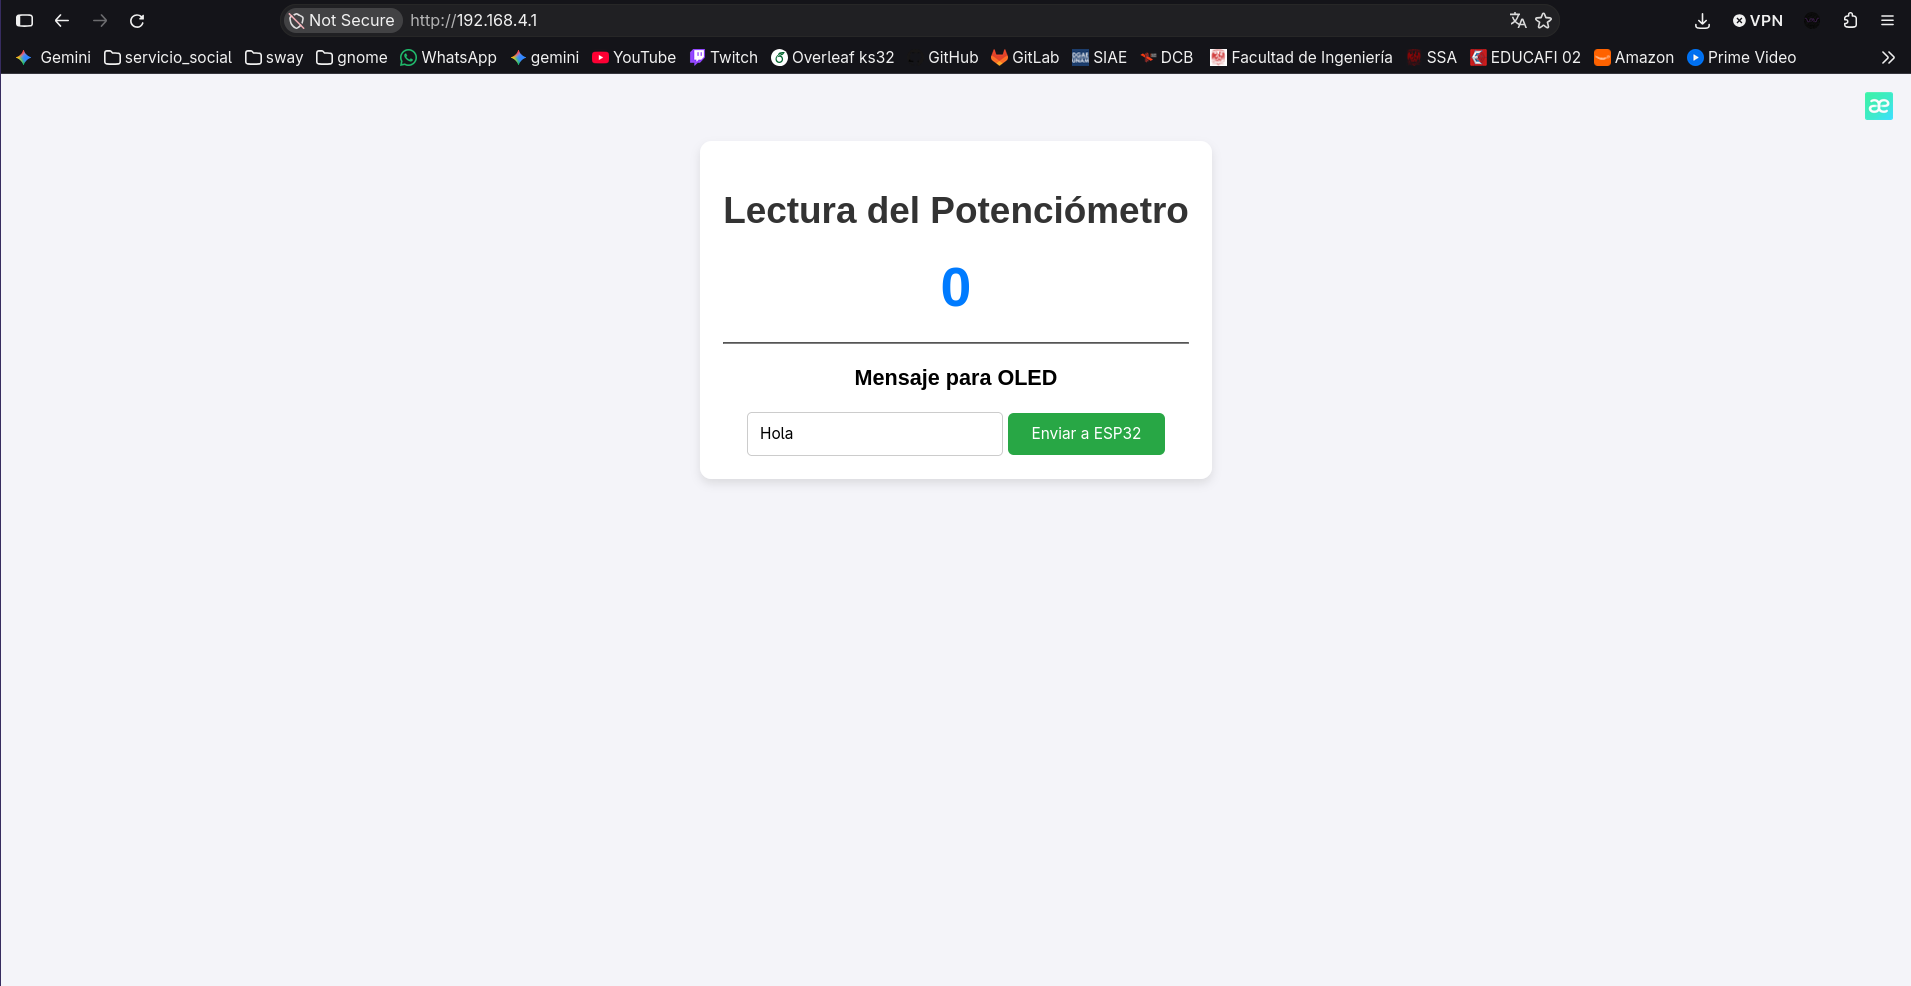
\includegraphics[width=\textwidth]{web_01.png}
        \caption{Página web al iniciar.}
    \end{subfigure}\hfill
    \begin{subfigure}[b]{0.4\textwidth}
        \centering
        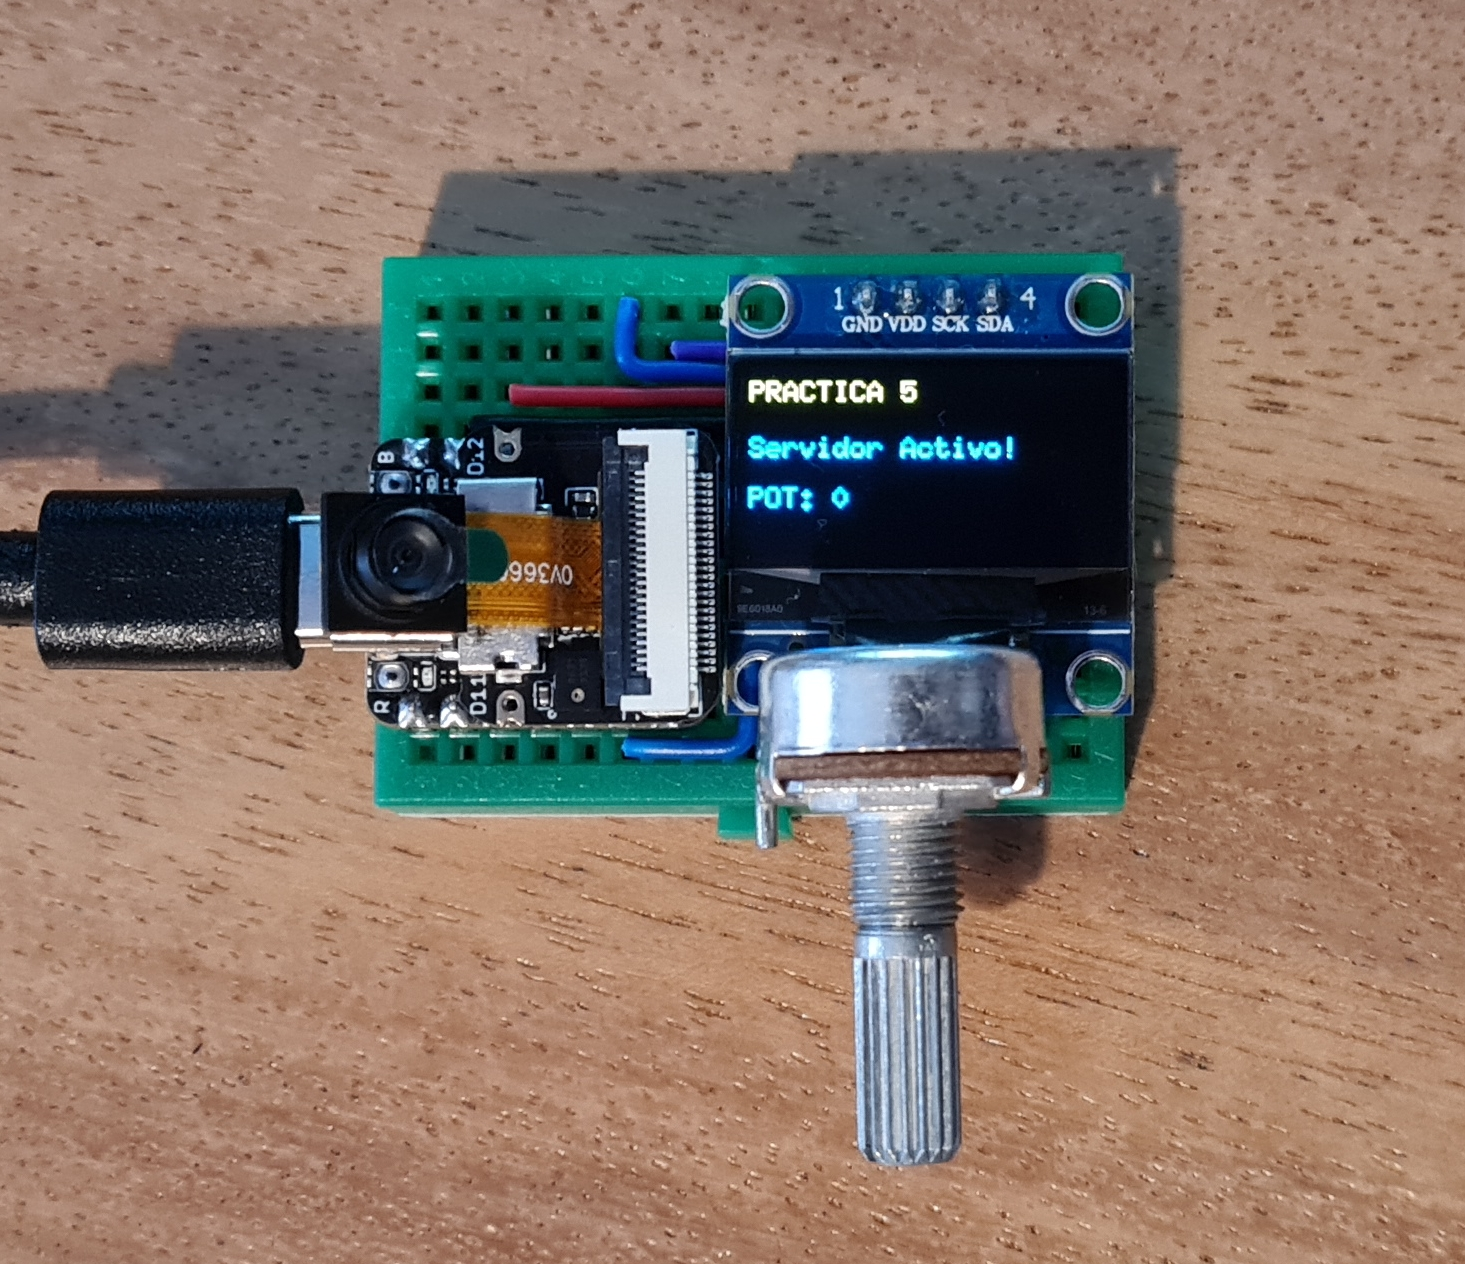
\includegraphics[width=\textwidth]{esp_01.jpg}
        \caption{OLED asociada.}
    \end{subfigure}
    \caption{Conexión inicial y servidor activo.}
    \label{fig:pareja01}
\end{figure}

En la siguiente figura se muestra la actualización de la lectura del
potenciómetro. La página web muestra el valor 3359 y la pantalla OLED muestra
el valor 3347, esto debido a que la lectura del ADC se realiza cada 500 ms y
puede variar ligeramente entre una lectura y otra. Cabe destacar que hasta este
momento aún no se ha enviado ningún mensaje desde la página web, por lo que la
OLED solo muestra el valor del potenciómetro.

\begin{figure}[H]
    \centering
    \begin{subfigure}[b]{0.55\textwidth}
        \centering
        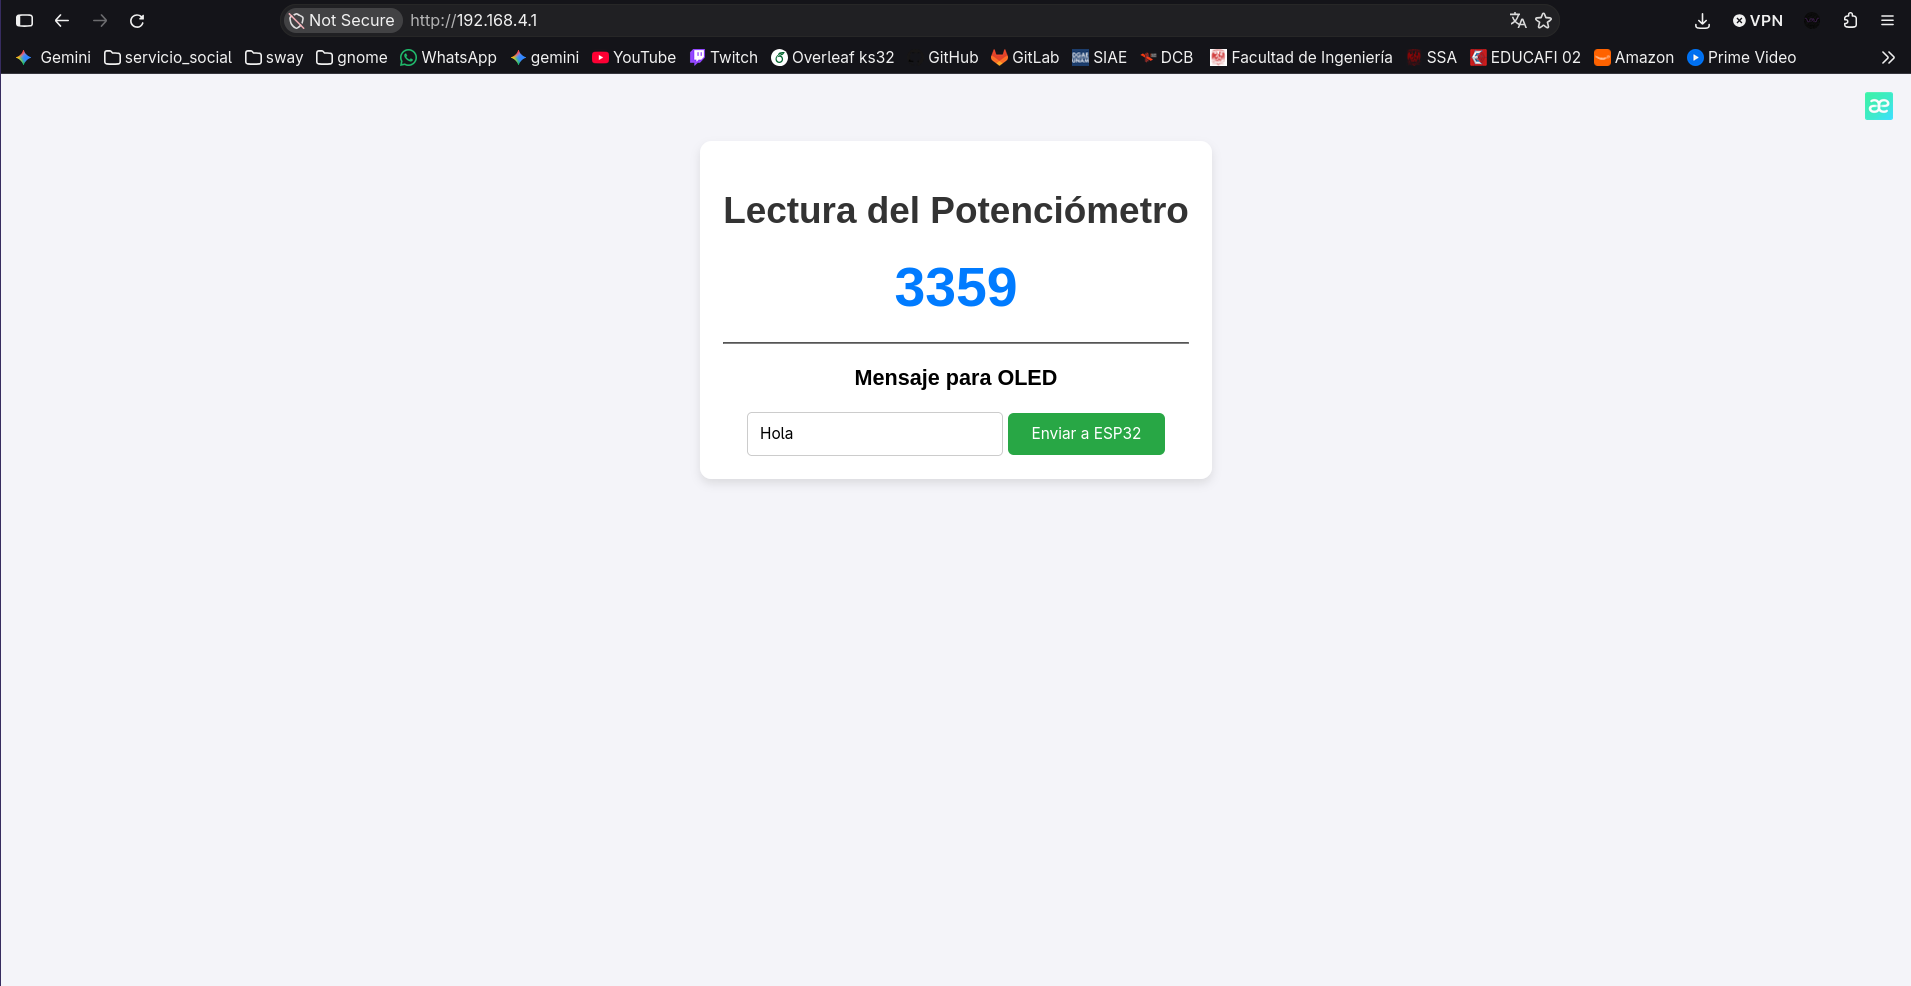
\includegraphics[width=\textwidth]{web_02.png}
        \caption{Lectura mostrada: 3359.}
    \end{subfigure}\hfill
    \begin{subfigure}[b]{0.4\textwidth}
        \centering
        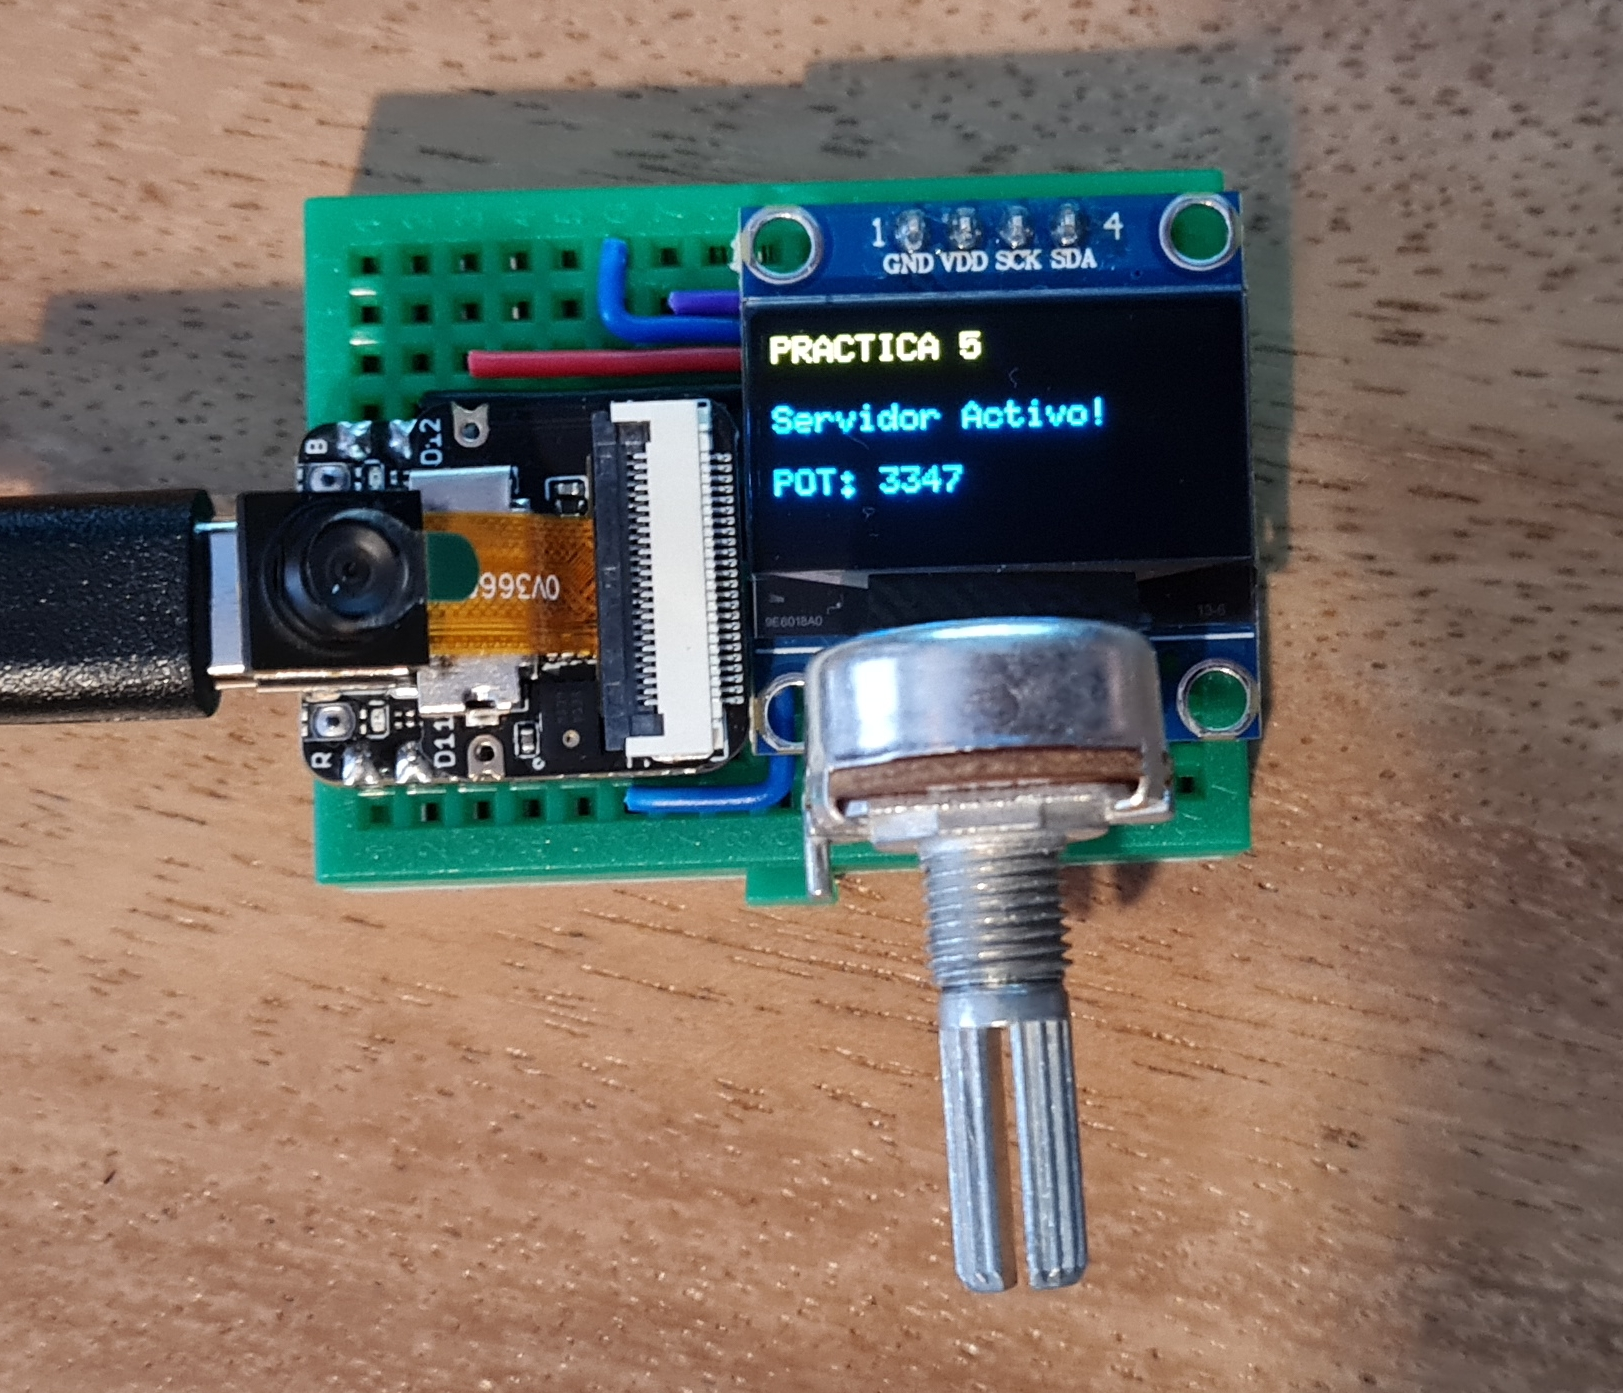
\includegraphics[width=\textwidth]{esp_02.jpg}
        \caption{Lectura en la OLED: 3347.}
    \end{subfigure}
    \caption{Actualización de la lectura del potenciómetro.}
    \label{fig:pareja02}
\end{figure}

Finalmente, en la siguiente figura se muestra la página web con el mensaje
\texttt{prueba1} escrito en el campo de texto y la pantalla OLED mostrando el
mismo mensaje junto con la lectura del potenciómetro. Esto demuestra que la
comunicación bidireccional mediante WebSocket funciona correctamente,
permitiendo enviar mensajes desde el navegador al ESP32 y viceversa.

\begin{figure}[H]
    \centering
    \begin{subfigure}[b]{0.55\textwidth}
        \centering
        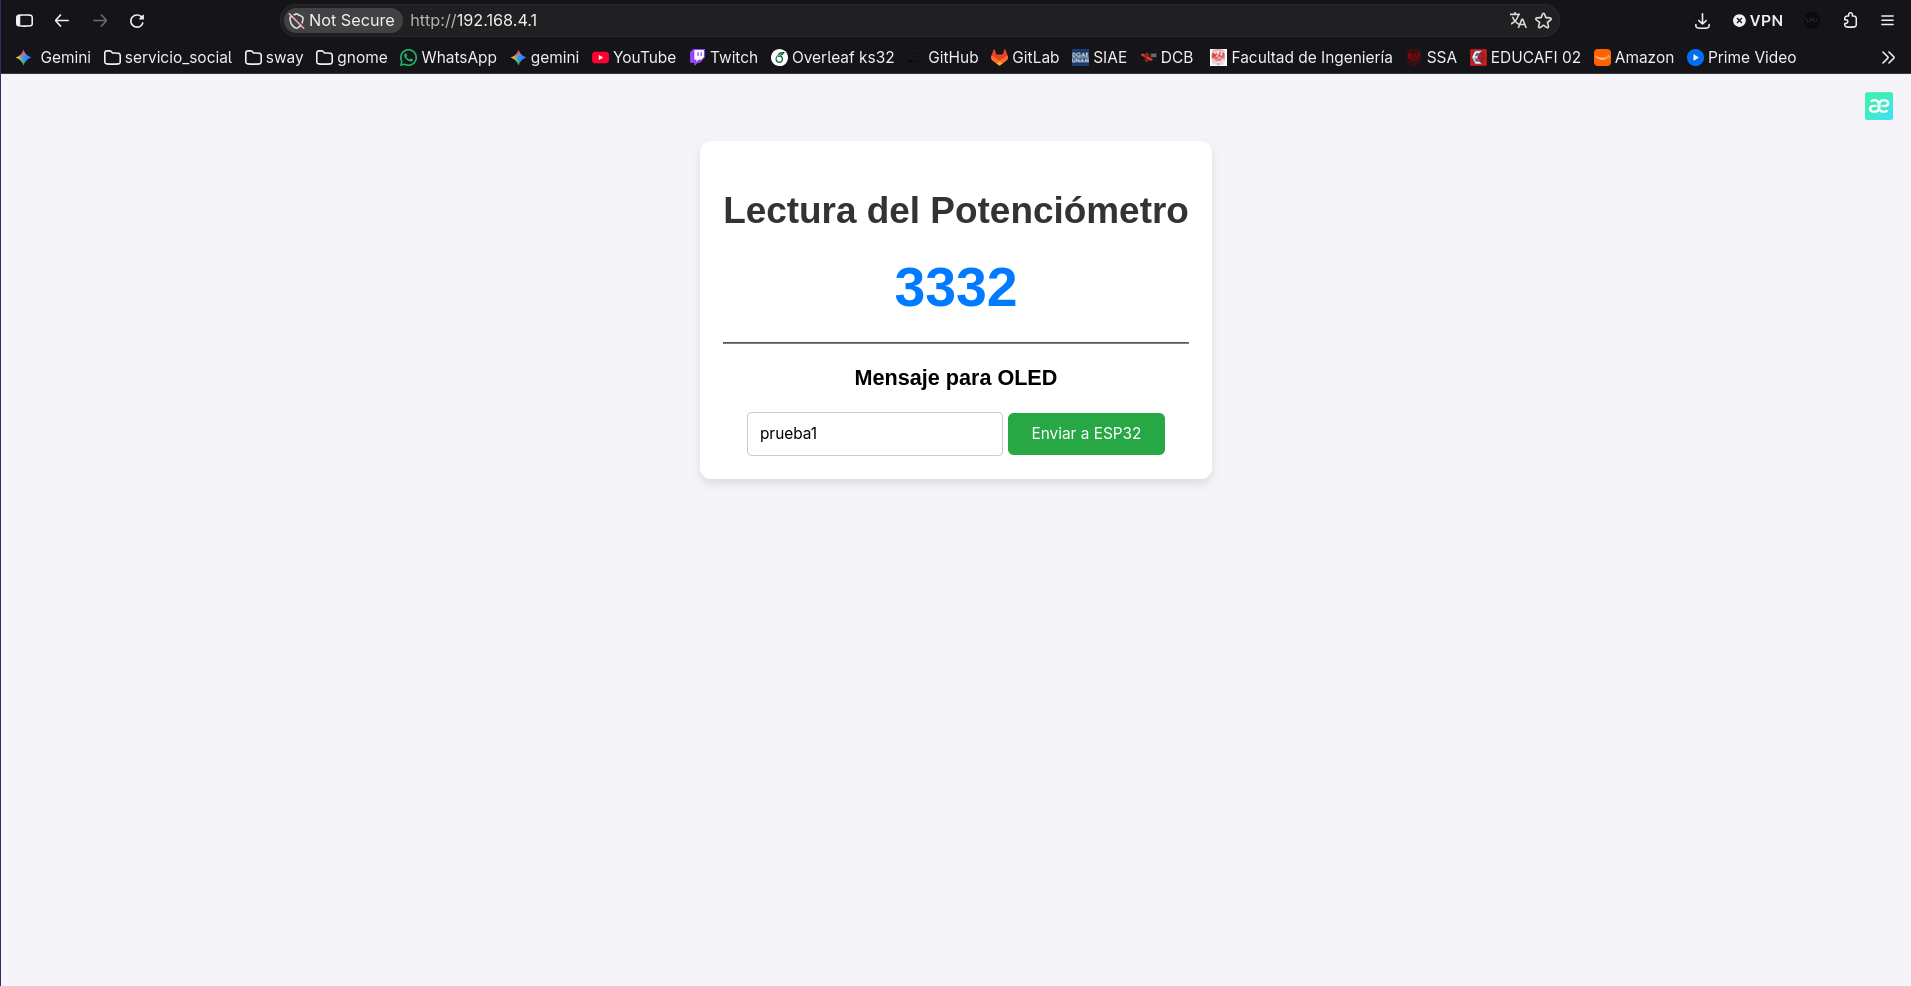
\includegraphics[width=\textwidth]{web_03.png}
        \caption{Mensaje escrito en la página: prueba1.}
    \end{subfigure}\hfill
    \begin{subfigure}[b]{0.4\textwidth}
        \centering
        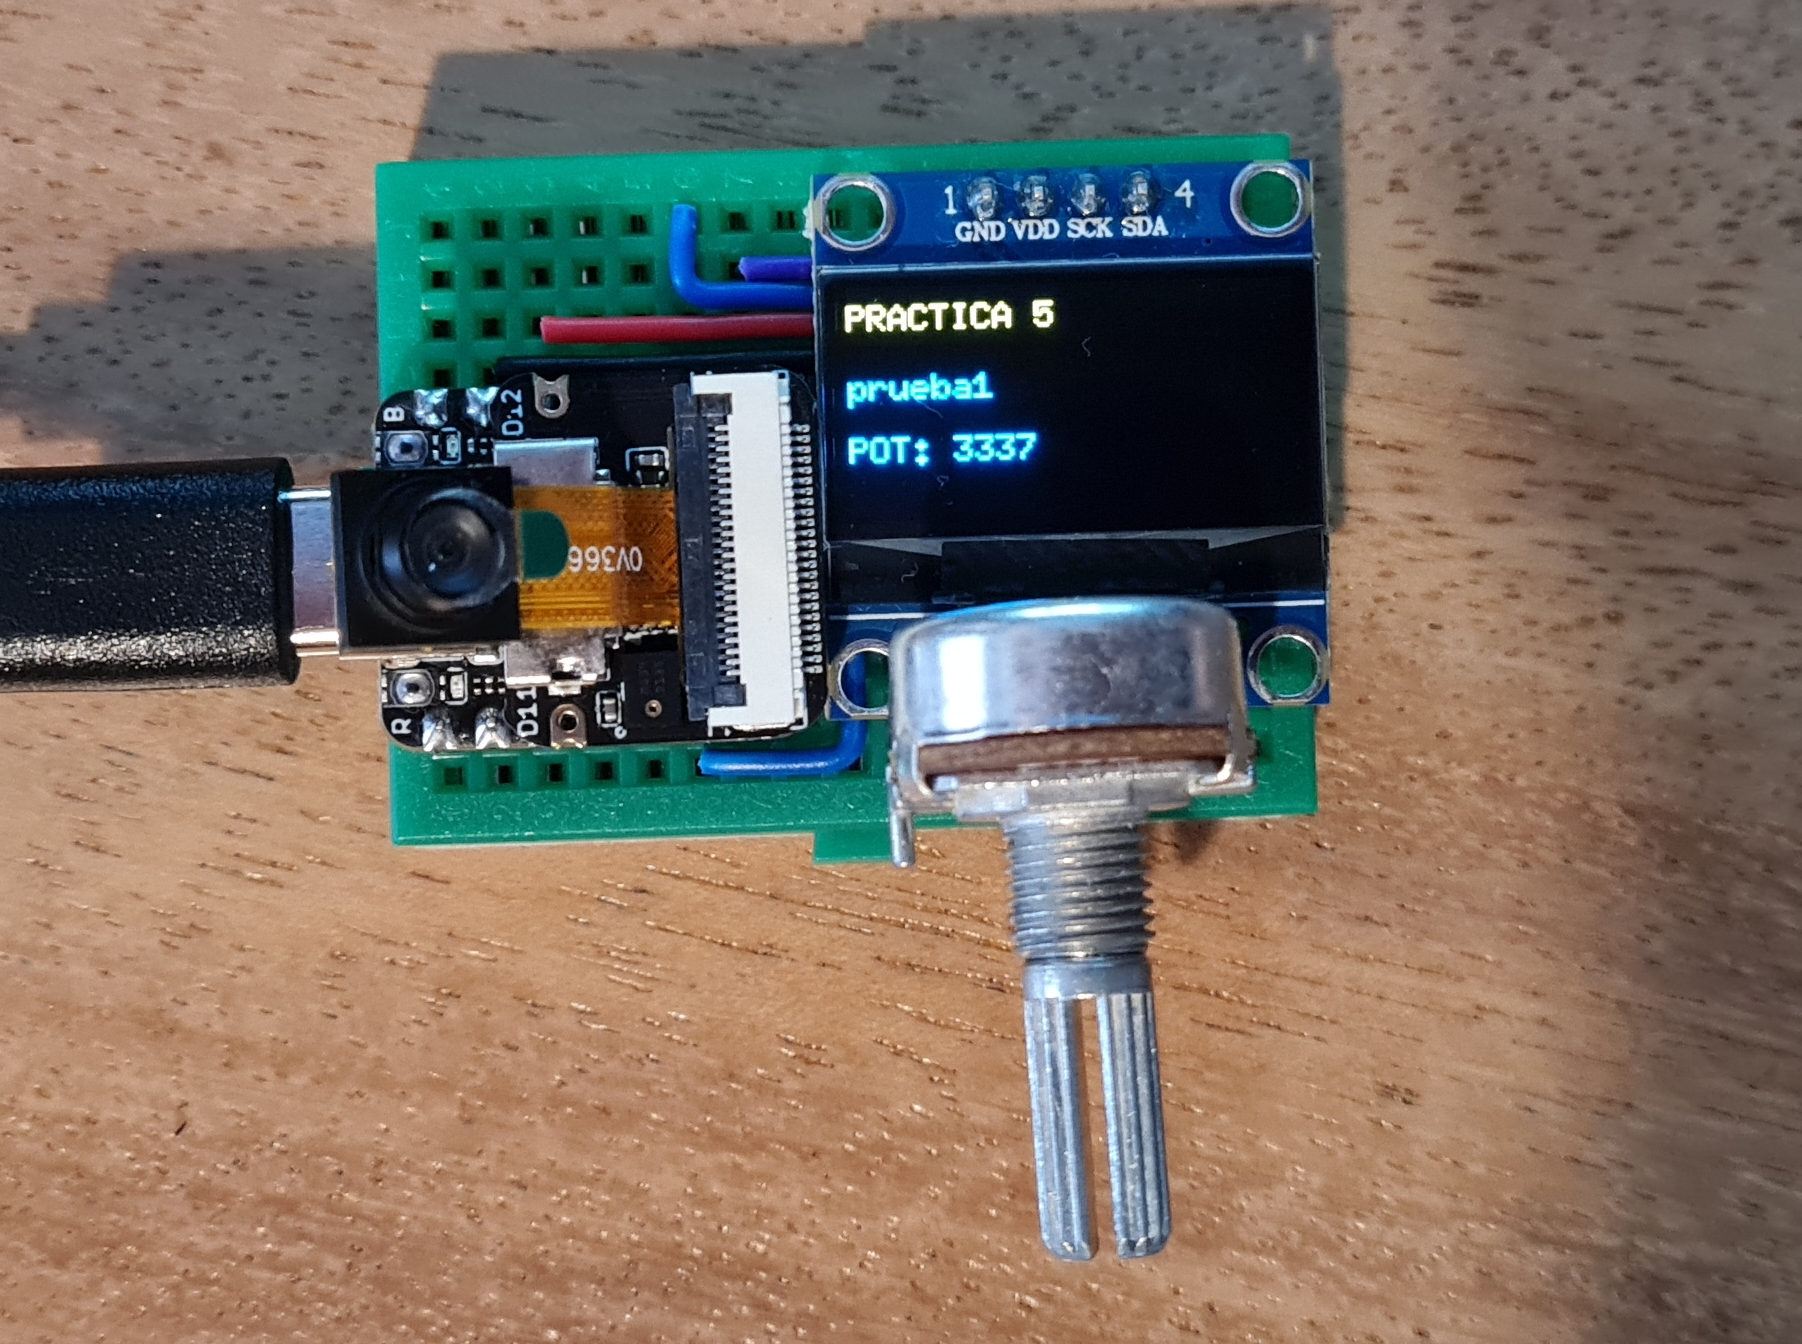
\includegraphics[width=\textwidth]{esp_03.jpg}
        \caption{Mensaje mostrado en la OLED junto con la lectura del potenciómetro.}
    \end{subfigure}
    \caption{Envío de mensaje desde el navegador al ESP32 mediante WebSocket.}
    \label{fig:pareja03}
\end{figure}

\textbf{Análisis del envío de mensajes.} La recepción de tramas de longitud desconocida y la reserva de \texttt{len + 1} bytes son importantes para evitar desbordamientos y garantizar que el texto sea una cadena C válida. La conexión WebSocket también permite que la página envíe datos al ESP32 sin abrir otra solicitud HTTP. Como la página usa UTF-8, los acentos y la letra ñ llegan como varios bytes; para mostrarlos correctamente sería necesario utilizar una fuente de la OLED que contenga esos caracteres.

\textbf{Análisis de los protocolos.} HTTP resulta adecuado para entregar la página inicial, mientras que WebSocket mantiene un canal TCP persistente, bidireccional y confiable para las mediciones y los mensajes. UDP tendría menor sobrecarga y latencia, pero no garantiza entrega ni orden, y el navegador no puede abrir directamente sockets UDP arbitrarios desde JavaScript. Por ello, WebSocket fue la opción más apropiada para esta interfaz web.

\section*{\centering \fontsize{14}{17}\sffamily\selectfont Conclusiones}

La práctica permitió integrar adquisición analógica, conectividad WiFi, HTTP, WebSocket y una pantalla OLED. El ESP32 creó la red AP, entregó la página, actualizó el valor del potenciómetro y recibió mensajes desde el navegador.

HTTP es adecuado para entregar la página inicial; WebSocket mantiene una conexión TCP persistente y bidireccional para enviar mediciones y mensajes. UDP tendría menor sobrecarga, pero no garantiza entrega ni orden y no puede utilizarse directamente desde JavaScript en el navegador.

Como cualquier dispositivo de la red AP podría enviar texto, una aplicación
real debería incorporar autenticación, cifrado, validación de mensajes y
control de acceso. Esta solución puede aplicarse en monitoreo ambiental,
automatización doméstica, mantenimiento y control remoto de actuadores.

\newpage
\textbf{NOTA: Si se desea consultar el código fuente completo del proyecto, se puede acceder al repositorio de GitHub en la siguiente dirección:} \url{https://github.com/lethalSopaper/laboratorio_sistemas_embebidos}

\end{document}
